\chapter{SUSTAINABLE DEVELOPMENT GOALS (SDGs)}

\section{Overview of SDGs}

The United Nations approved the Sustainable Development Goals (SDGs) popularly known as the Global Goals in 2015 as a universal call to end poverty, protect the planet and secure peace and prosperity to all by the year 2030. These 17 goals are closely connected, and it should be emphasized that the accomplishment of one field inevitably affects the results in other areas, and to achieve the real sustainability, the social, economic and environmental aspects should be considered with the necessary equilibrium.
	
	Engaging in the sphere of engineering research and development, the understanding of how a technical solution promotes the solution of the global issues is the primary concern. This project is called User-Friendly Autonomous Parcel Delivery System with Adaptive Navigation; it corresponds to several SDGs because it successfully incorporates robotics and intelligent automation into the world of healthcare, education, and industrial infrastructure.
\begin{figure}[H]
	\centering
	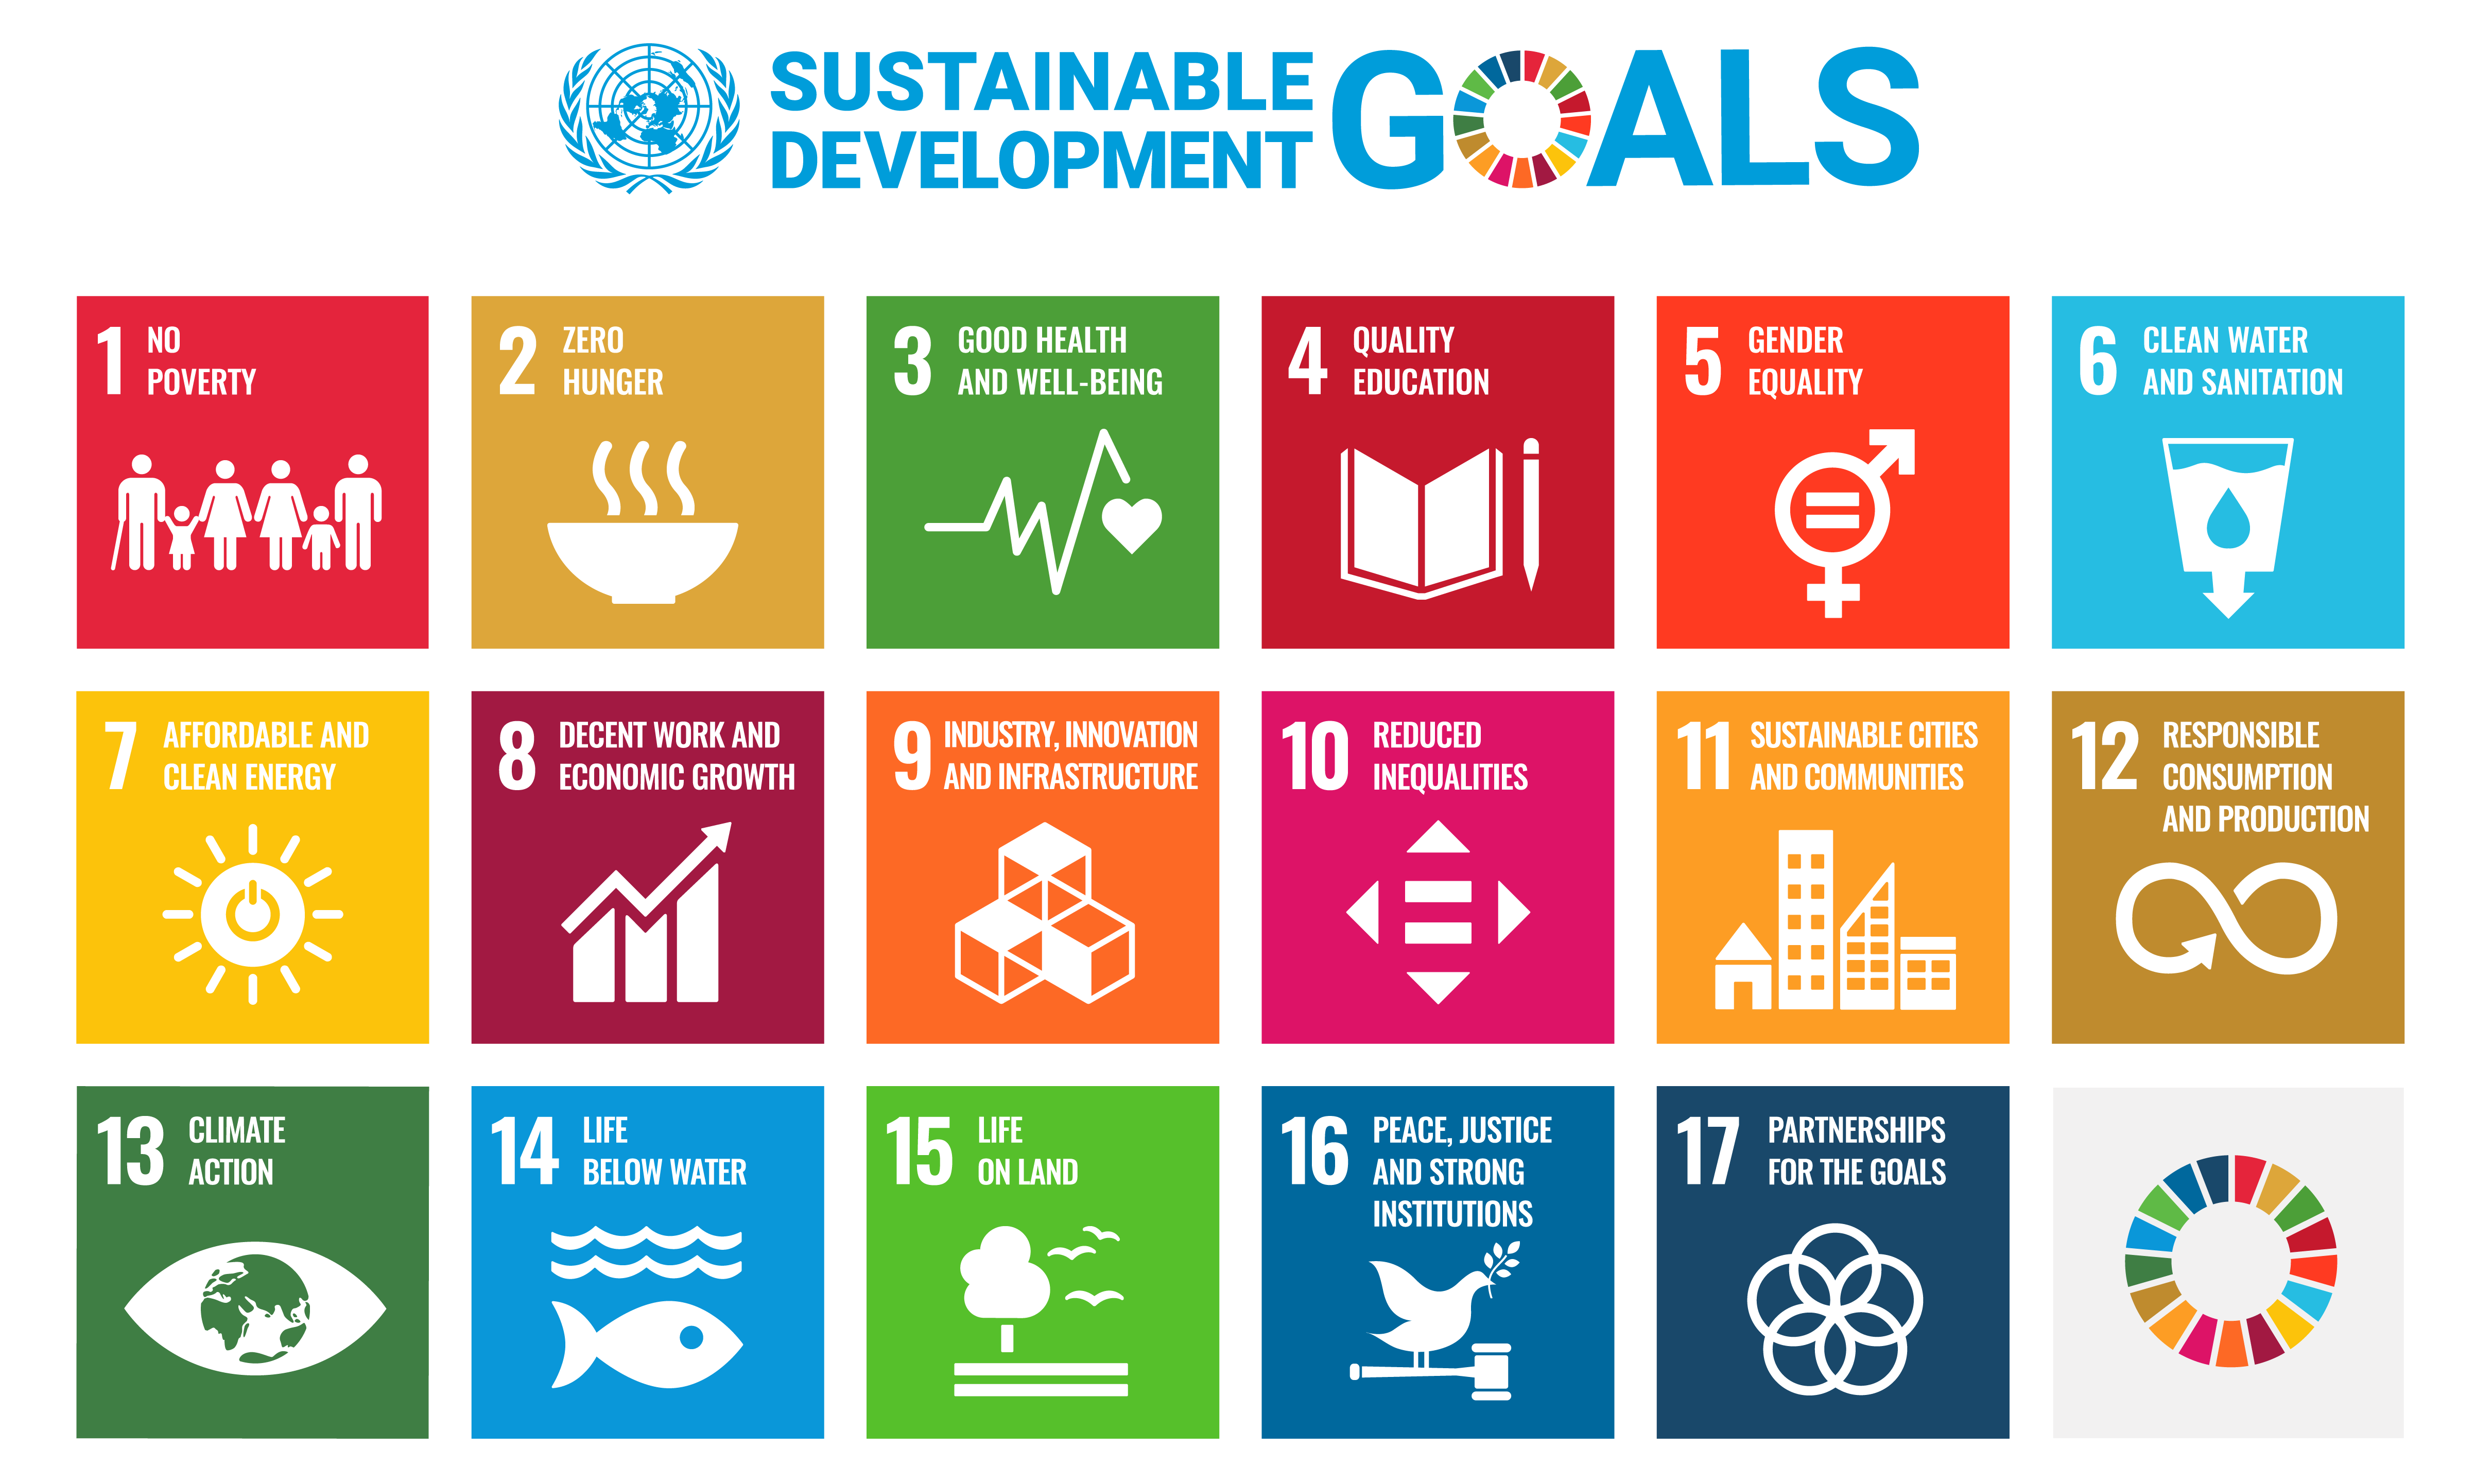
\includegraphics[width=0.85\textwidth]{SDGs.png}
	\caption{United Nations 17 Sustainable Development Goals Framework~\cite{un2015sdgs}}
	\label{fig:sdg_overview}
\end{figure}

\section{Alignment of Project with SDGs}

\subsection{SDG 3: Good Health and Well-Being}

The healthcare industry is one of the main areas of application of the suggested autonomous delivery system. The SDG~3 is relevant to the project in the following ways:

\begin{itemize}
	\item \textbf{Infection Control:}
	
	The robot can transport medicines, laboratory samples, and medical supplies without involving human movements, which is why it reduces the needless human movement in the high-risk areas and, consequently, minimizes the chances of cross-contamination and transmitting infectious diseases.
	
	\item \textbf{Operational Efficiency:} 	Relocating logistical duties that are repetitive to the healthcare workers will enable them to pay more attention to the patients, lessening the workload burden and enhancing the overall health services quality.
	
	\item \textbf{Safety in Medical Logistics:}	The system guarantees a regulated and trusted approach of handling sensitive materials as well as the integrity of samples and forms of transport.
\end{itemize}

\begin{figure}[H]
	\centering
	
\includegraphics[width=0.3\textwidth]{sdg3.png}
	\caption{SDG 3: Good Health and Well-Being}
	\label{fig:sdg3_health}
\end{figure}

\subsection{SDG 4: Quality Education}

The proposed system also supports SDG~4 by enhancing operational efficiency and learning opportunities within educational institutions:

\begin{itemize}
	\item \textbf{Campus Automation:} 
	The robot also helps in the transportation of documents, books, and laboratory equipment across the various departments, enhancing the logistics in the institution and minimizing the administration delays.
	
	\item \textbf{Practical Engineering Application:} 
	Being a research based project, it is an effective tool that enables the learner to learn ROS~2, autonomous navigation, and path planning, which is a gap between theory and practice.
\end{itemize}

\begin{figure}[H]
	\centering
	
\includegraphics[width=0.3\textwidth]{sdg4.png}
	\caption{SDG 4: Quality Education ~\cite{unsdg4}}
	\label{fig:sdg4_education}
\end{figure}

\subsection{SDG 9: Industry, Innovation, and Infrastructure}

Innovation and infrastructure development form the core of this Final Year Project (FYP). The proposed system contributes to SDG~9 in the following ways:

\begin{itemize}
		\item \textbf{Technological Advancement:} Application of the Robot Operating System (ROS 2) and new perception devices including LiDAR and RGB-D cameras is an important milestone towards intelligent and autonomous internal logistics.
		
	
	\item \textbf{Scalable Industrial Solutions:} 
	
	The modular structure enables both large-scale warehouse, hospital, and industrial facilities deployments as well as supporting robust and innovative infrastructures.
	
		
	\item \textbf{Efficiency in Logistics:}	The system enhances reliability or productivity within the commercial and industrial settings by minimizing human error and manual handling of products when it comes to indoor transportation.
	
\end{itemize}

\begin{figure}[H]
	\centering
	
\includegraphics[width=0.3\textwidth]{sdg9.png}
	\caption{SDG 9: Industry, Innovation and Infrastructure }
	\label{fig:sdg9_innovation}
\end{figure}

\subsection{SDG 11: Sustainable Cities and Communities}

The project supports the vision of smart and sustainable communities through intelligent automation.

\begin{itemize}
	\item \textbf{Smart Campus and Office Integration:} 
	The automation of in-door delivery allows reducing the human overload on the system, and enhances workplace and learning area organization.
	
	
	\item \textbf{Sustainable Resource Management:} 
	The electric robotic platform that is run by battery reduces the carbon footprint to the traditional methods of transport which use either manual or fuel-powered methods which helps in creating cleaner and sustainable living environments.
	
\end{itemize}

\begin{figure}[H]
	\centering
	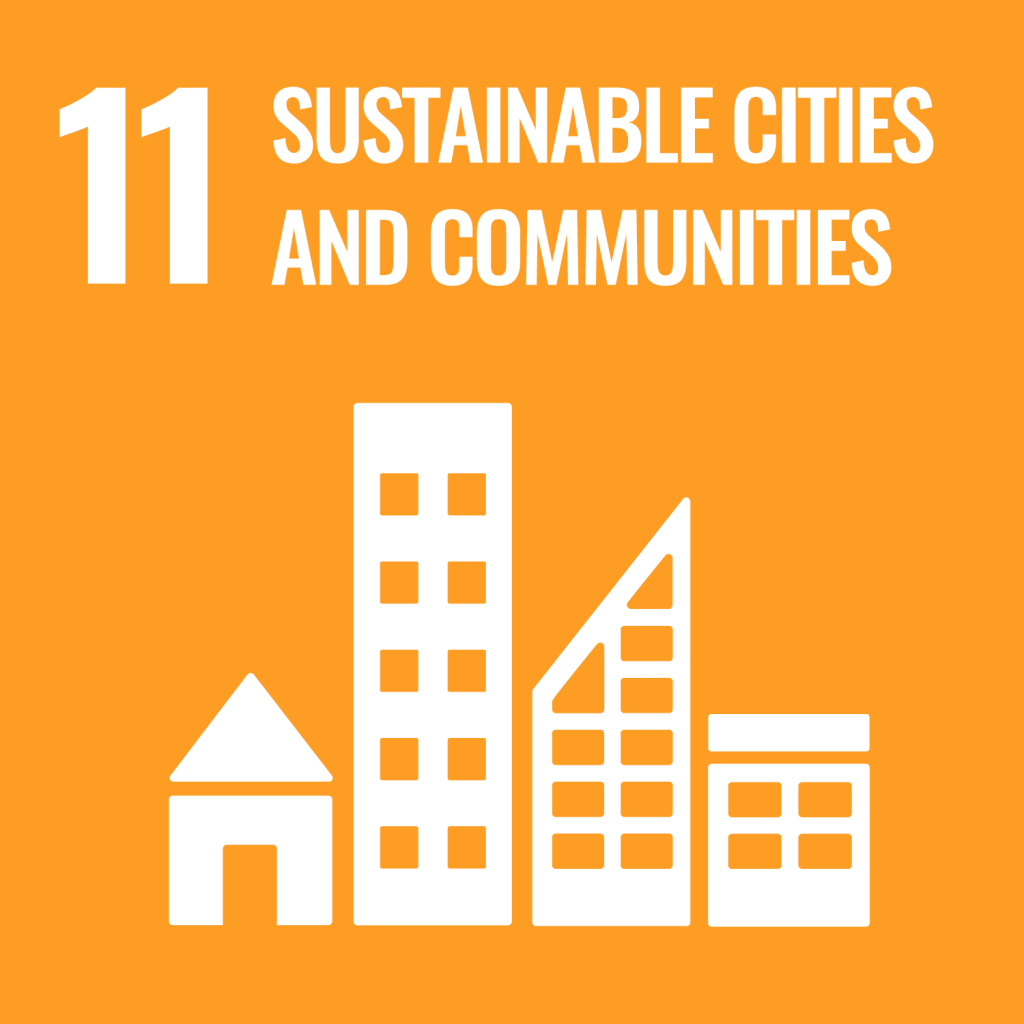
\includegraphics[width=0.3\textwidth]{sdg11.png}
	\caption{SDG 11: Sustainable Cities and Communities~\cite{unsdg11}}
	\label{fig:sdg11_cities}
\end{figure}

\section{Implementation Summary Table}

Table~\ref{tab:sdg_implementation} summarizes the key contributions of the proposed system to the targeted Sustainable Development Goals.

\begin{table}[H]
	\centering
	\caption{Project Alignment with Sustainable Development Goals}
	\label{tab:sdg_implementation}
	\begin{tabular}{|c|p{4cm}|c|p{6.5cm}|}
		\hline
		\textbf{Sr. No} & \textbf{Targeted SDGs} & \textbf{Goal No.} & \textbf{Implementation Detail} \\
		\hline
		1 & Good Health \& Well-Being & SDG~3 & Reduces human contact in hospitals by autonomously transporting medicines and laboratory samples, minimizing cross-contamination. \\
		\hline
		2 & Quality Education & SDG~4 & Supports university logistics and provides a practical research platform for autonomous robotics and ROS~2-based learning. \\
		\hline
		3 & Industry, Innovation \& Infrastructure & SDG~9 & Implements a scalable ROS~2-based architecture for modernizing internal logistics in commercial and industrial sectors. \\
		\hline
		4 & Sustainable Cities \& Communities & SDG~11 & Promotes the ``Smart Campus'' concept by reducing indoor congestion and improving delivery efficiency through automation. \\
		\hline
	\end{tabular}
\end{table}

\section{Chapter Summary}

This chapter showed the socio-economic and environmental applicability of the suggested Autonomous Delivery Robot by matching it with the United Nations Sustainable Development Goals. The project can achieve SDG~3, SDG~4, SDG~9, and SDG~11, which makes it much more than a technical prototype, but a sustainable and socially responsible project. This direction will see the project go in line with the worldwide vision of safe healthcare systems, quality education, innovative industries, and smart and sustainable communities.
